\chapter{शुद्ध पदार्थ और मिश्रण}\label{ch:g6:pure-substances-and-mixtures}

मिनरल वॉटर की बोतल के लेबल पर लगभग एक दर्जन घुले हुए पदार्थों के नाम
लिखे होते हैं, साथ में उनकी मात्रा मिलीग्राम प्रति लीटर में। प्रयोगशाला के
शोधक से निकलने वाले पानी पर कोई नाम नहीं लिखा होता। दोनों स्वच्छ और
रंगहीन हैं, दोनों प्यास बुझाते हैं --- फिर भी उनमें से केवल एक ही वह है
जिसे रसायनज्ञ शुद्ध कहता है। यह अध्याय ``शुद्ध'' शब्द को उसका सटीक अर्थ
देता है, और दिखाता है कि कुछ भी चखे बिना \omterm{def:g6:pure-substances-and-mixtures:pure-substance}{शुद्ध पदार्थ} को \omterm{def:g6:pure-substances-and-mixtures:mixture}{मिश्रण} से कैसे
अलग पहचाना जाए।

\begin{recall}
\omterm{def:g2:mixing-and-dissolving:mix}{मिलाना} यानी अलग-अलग चीज़ों को एक साथ रखना; पानी में \omterm{def:g2:mixing-and-dissolving:dissolve}{घुलने} वाला ठोस द्रव
को स्वच्छ छोड़ता है, और वह स्वच्छ द्रव एक विलयन है
(\cref{ch:g2:mixing-and-dissolving})। \omterm{def:g6:pure-substances-and-mixtures:mixture}{मिश्रणों} को चालकर, निथारकर,
छानकर और \omterm{def:g3:separating-mixtures:evaporate}{वाष्पन} करके अलग किया जा सकता है
(\cref{ch:g3:separating-mixtures})। हर सामग्री के ऐसे गुण होते हैं जिन्हें
परखा जा सकता है: कठोर या नरम, पारदर्शी या नहीं, तैरती है या डूबती है
(\cref{ch:g1:materials-around-us})।
\end{recall}

\section{रासायनिक स्पीशीज़ और शुद्ध पदार्थ}

\begin{definition}[रासायनिक स्पीशीज़]\label{def:g6:pure-substances-and-mixtures:species}
\emph{रासायनिक स्पीशीज़}\index{रासायनिक स्पीशीज़} किसी पदार्थ का एक
विशेष प्रकार है, जिसका अपना नाम और अपने गुण होते हैं: पानी, चीनी,
नमक, ऑक्सीजन, एथेनॉल (शराब में पाया जाने वाला ऐल्कोहॉल), लोहा।
\end{definition}

\begin{definition}[शुद्ध पदार्थ]\label{def:g6:pure-substances-and-mixtures:pure-substance}
\emph{शुद्ध पदार्थ}\index{शुद्ध पदार्थ} केवल एक ही \omterm{def:g6:pure-substances-and-mixtures:species}{रासायनिक स्पीशीज़}
से बना होता है, और किसी चीज़ से नहीं: आसुत जल, चीनी का एक क्रिस्टल,
शुद्ध सोने की अँगूठी।
\end{definition}

\begin{definition}[मिश्रण]\label{def:g6:pure-substances-and-mixtures:mixture}
\emph{मिश्रण}\index{मिश्रण} में कई \omterm{def:g6:pure-substances-and-mixtures:species}{रासायनिक स्पीशीज़} होती हैं। \omterm{def:g4:air-a-mixture-of-gases:air}{वायु},
समुद्र का पानी, मिनरल वॉटर, दूध, ग्रेनाइट और संतरे का रस मिश्रण हैं।
\end{definition}

\begin{remark}[रोज़मर्रा की भाषा में शुद्ध]\label{rem:g6:pure-substances-and-mixtures:everyday}
``शुद्ध संतरे का रस'' लिखे डिब्बे का अर्थ है कि रस में कुछ मिलाया नहीं गया।
रसायनज्ञ के लिए वह रस फिर भी एक \omterm{def:g6:pure-substances-and-mixtures:mixture}{मिश्रण} है: पानी, शर्कराएँ, अम्ल, विटामिन,
रंग और सुगंध, यानी अनेक \omterm{def:g6:pure-substances-and-mixtures:species}{रासायनिक स्पीशीज़}। ``पहाड़ों का शुद्ध पानी''
भी एक \omterm{def:g6:pure-substances-and-mixtures:mixture}{मिश्रण} है: घुले हुए लवणों वाला पानी।
\end{remark}

\begin{omfigure}
\begin{tikzpicture}[font=\small, level distance=1.55cm,
    box/.style={draw=omDef, fill=omDef!6, rounded corners=2pt, align=center,
      inner sep=4pt},
    level 1/.style={sibling distance=7.2cm},
    level 2/.style={sibling distance=3.6cm},
    edge from parent/.style={draw, thick, omDef, ->}]
  \node[box] {द्रव्य}
    child {node[box] {शुद्ध पदार्थ\\ \footnotesize एक रासायनिक स्पीशीज़}
      child {node[box, draw=black!40, fill=white] {आसुत जल,\\ नमक, लोहा}}}
    child {node[box] {मिश्रण\\ \footnotesize कई रासायनिक स्पीशीज़}
      child {node[box] {समांगी\\ \footnotesize हर जगह एक-सा रूप}
        child {node[box, draw=black!40, fill=white] {नमकीन पानी,\\ वायु}}}
      child {node[box] {विषमांगी\\ \footnotesize हिस्से दिखते हैं}
        child {node[box, draw=black!40, fill=white] {गंदला पानी,\\ ग्रेनाइट}}}};
\end{tikzpicture}

{\small द्रव्य का वर्गीकरण। सबसे नीचे के खाने हर प्रकार के उदाहरण देते हैं।}
\end{omfigure}

\section{समांगी और विषमांगी मिश्रण}

\begin{definition}[समांगी और विषमांगी मिश्रण]\label{def:g6:pure-substances-and-mixtures:homogeneous}
कोई \omterm{def:g6:pure-substances-and-mixtures:mixture}{मिश्रण} \emph{समांगी मिश्रण}\index{समांगी मिश्रण} होता है
जब उसके अलग-अलग हिस्से आँख से, आवर्धक लेंस से भी, अलग-अलग नहीं पहचाने
जा सकते: वह हर जगह एक-सा दिखता है। वह
\emph{विषमांगी मिश्रण}\index{विषमांगी मिश्रण} होता है जब कम से
कम दो अलग-अलग हिस्से दिखाई दें।
\end{definition}

\begin{example}[चार मिश्रण]\label{ex:g6:pure-substances-and-mixtures:four}
नमकीन पानी और \omterm{def:g4:air-a-mixture-of-gases:air}{वायु} समांगी हैं: उनके हिस्से दिखाई नहीं देते। पानी पर तेल
विषमांगी है: दो परतें। गंदला पानी विषमांगी है: उसमें कण तैरते हैं और नीचे
बैठ जाते हैं। गूदे वाला संतरे का रस विषमांगी है: गूदे के टुकड़े दिखाई
देते हैं।
\end{example}

\begin{omfigure}
\begin{tikzpicture}[font=\small, scale=1.15]
  \pic[transform shape] at (0,0) {beaker={0.7}{omWater!80}};
  \node[anchor=north, align=center] at (0,-0.15) {नमकीन पानी:\\ समांगी};
  \pic[transform shape] at (2.6,0) {beaker={0.7}{omWater!80}};
  \fill[yellow!55!orange!60] (1.8,1.05) rectangle (3.4,1.4);
  \draw[omGlass, line width=0.7pt] (1.8,1.05) -- (1.8,1.4) (3.4,1.05) -- (3.4,1.4);
  \node[anchor=north, align=center] at (2.6,-0.15) {पानी पर तेल:\\ विषमांगी};
  \pic[transform shape] at (5.2,0) {beaker={0.7}{brown!25}};
  \foreach \x/\y in {4.6/0.3,4.9/0.7,5.3/0.5,5.6/1.0,5.0/1.1,5.4/0.2,5.8/0.6}
    \fill[brown!65] (\x,\y) circle (0.04);
  \fill[brown!60] (4.4,0) rectangle (6.0,0.12);
  \node[anchor=north, align=center] at (5.2,-0.15) {गंदला पानी:\\ विषमांगी};
  \pic[transform shape] at (7.8,0) {beaker={0.7}{orange!45}};
  \foreach \x/\y in {7.3/0.35,7.6/0.8,8.0/0.5,8.3/1.0,7.7/1.15,8.2/0.25,7.45/0.65}
    \fill[orange!80!brown] (\x,\y) ellipse (0.08 and 0.03);
  \node[anchor=north, align=center] at (7.8,-0.15) {गूदे वाला रस:\\ विषमांगी};
\end{tikzpicture}

{\small एक समांगी और तीन \omterm{def:g6:pure-substances-and-mixtures:homogeneous}{विषमांगी मिश्रण}।}
\end{omfigure}

\begin{omfigure}
\begin{minipage}[b]{0.48\linewidth}\centering
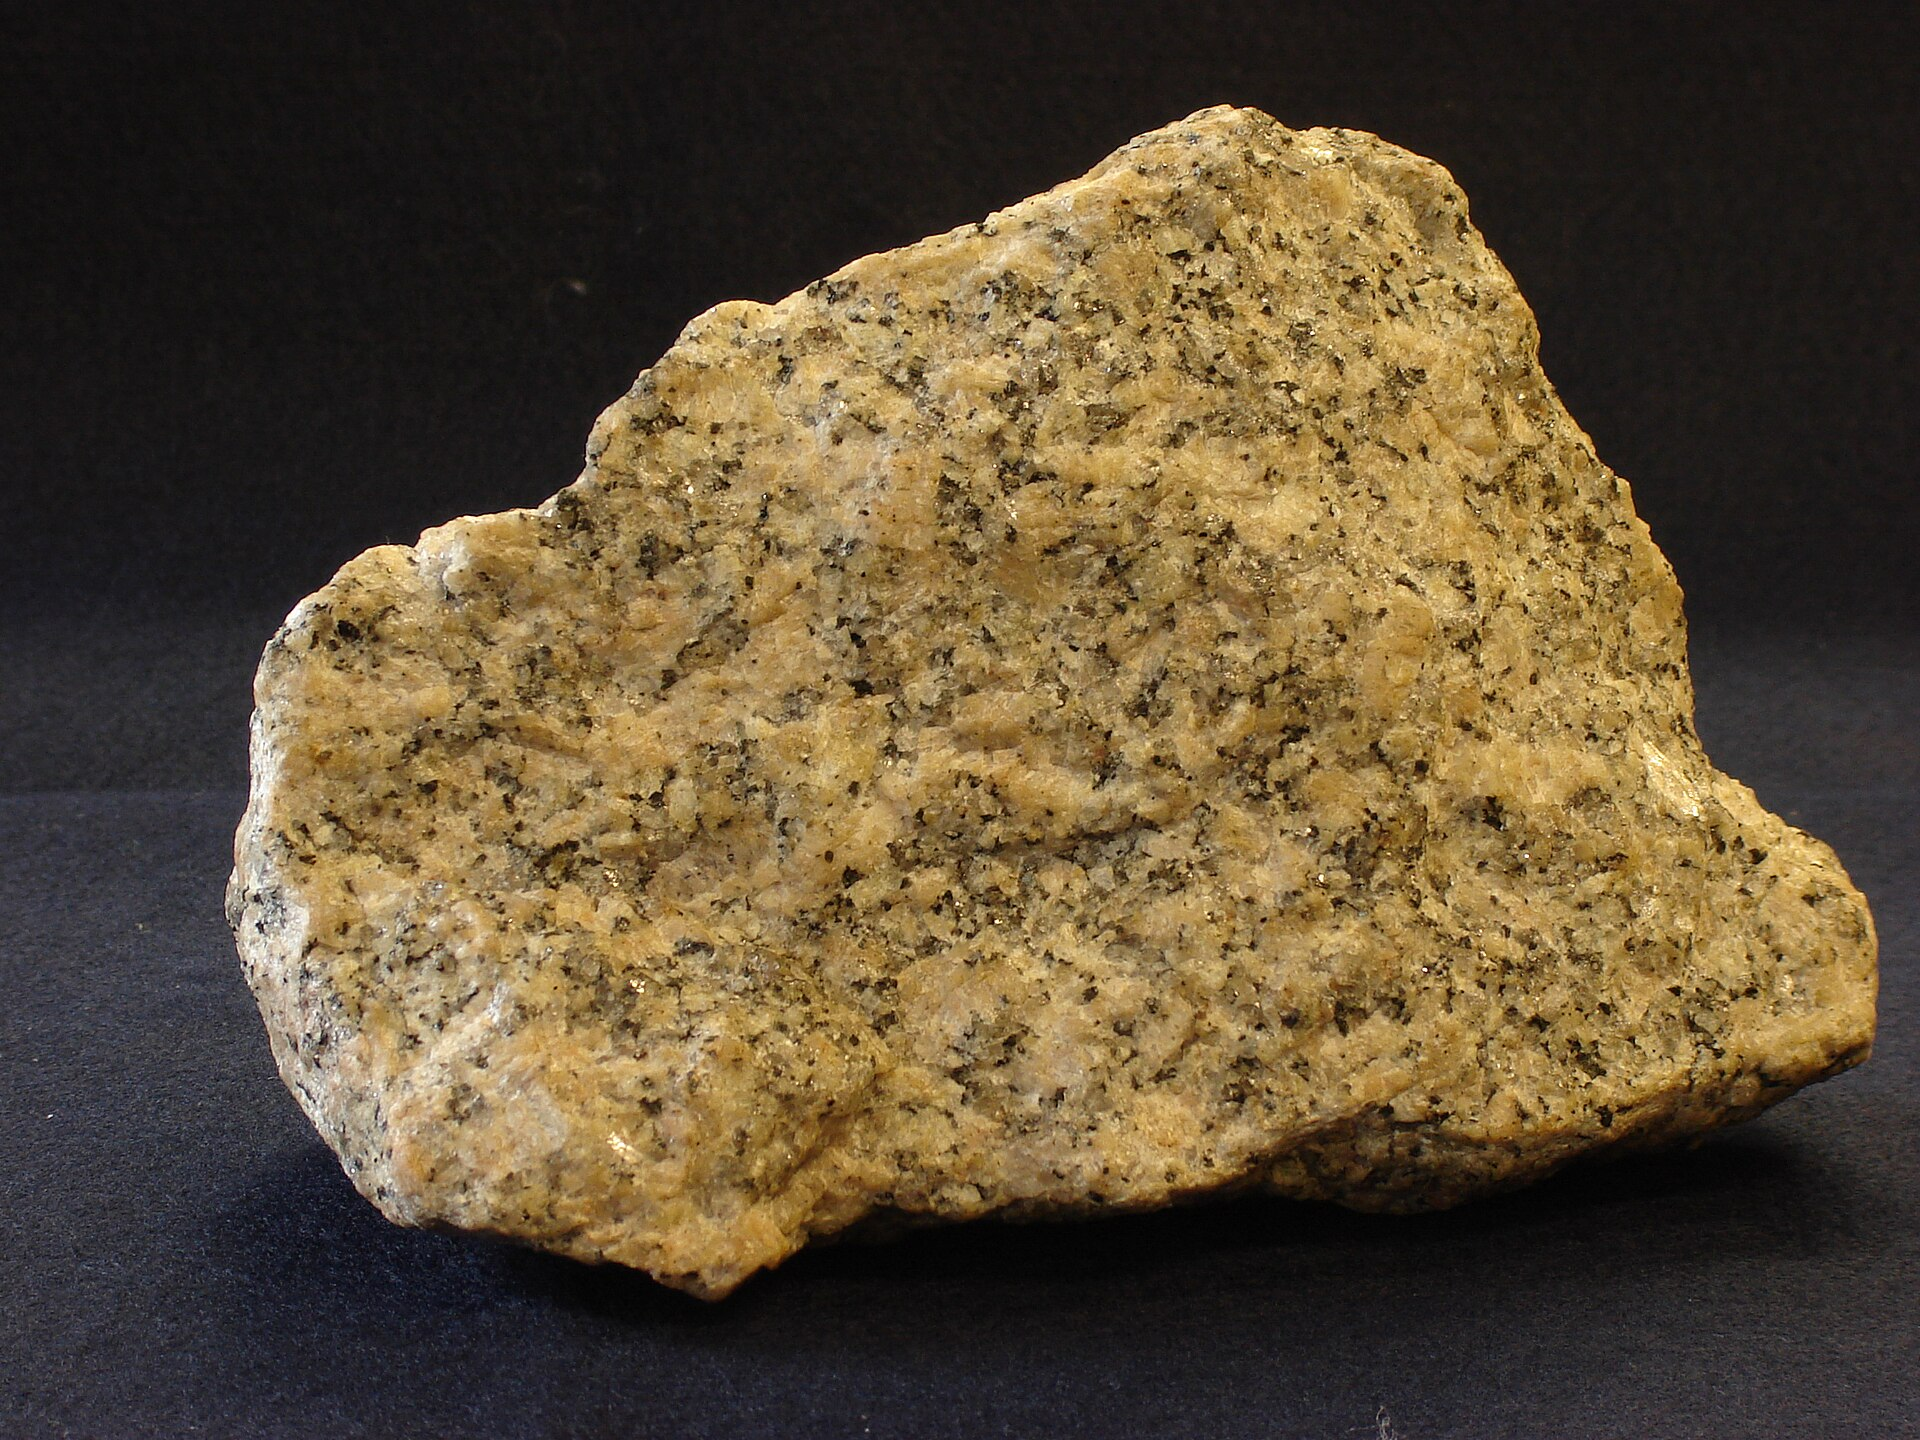
\includegraphics[width=\linewidth,height=4.6cm,keepaspectratio]{images/book1/granite.jpg}

{\small ग्रेनाइट: तीन-चार अलग-अलग खनिजों के कण दिखते हैं। एक विषमांगी
ठोस। फ़ोटो: एउरिको ज़िम्ब्रेस, CC BY-SA 2.0 br।}
\end{minipage}\hfill
\begin{minipage}[b]{0.48\linewidth}\centering
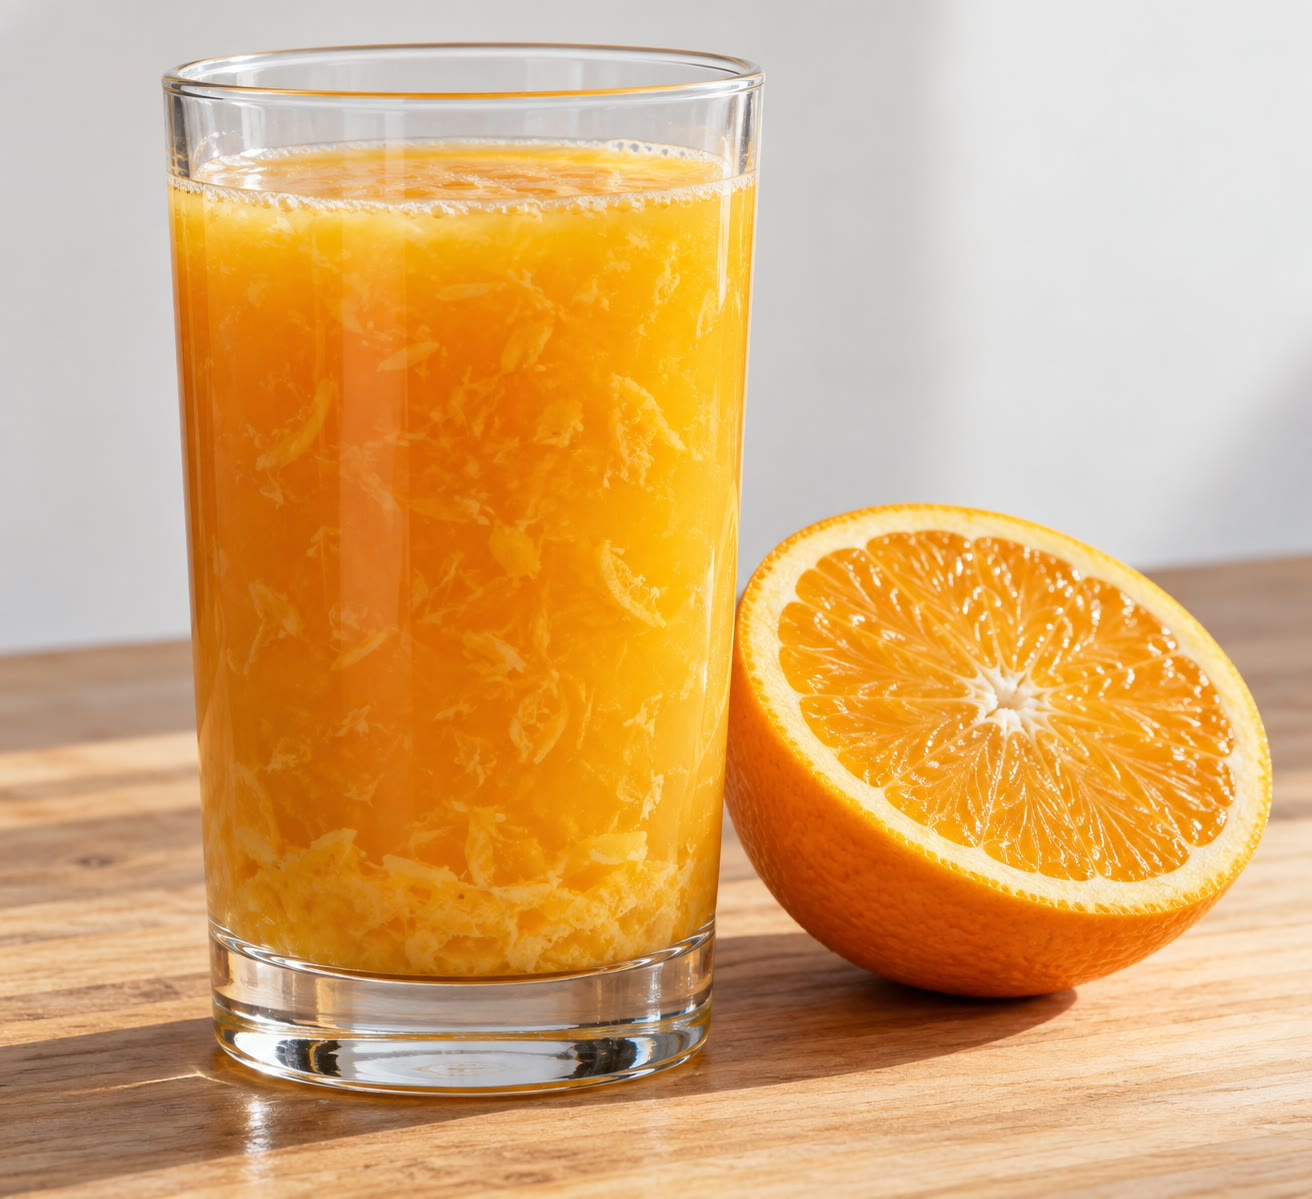
\includegraphics[width=\linewidth,height=4.6cm,keepaspectratio]{images/book1/ai/g6-orange-juice.jpg}

{\small गूदे वाला संतरे का रस: एक \omterm{def:g6:pure-substances-and-mixtures:homogeneous}{विषमांगी मिश्रण}।}
\end{minipage}
\end{omfigure}

\begin{remark}[समांगी का अर्थ शुद्ध नहीं]\label{rem:g6:pure-substances-and-mixtures:not-pure}
नमकीन पानी बिल्कुल शुद्ध पानी जैसा दिखता है। \omterm{def:g6:pure-substances-and-mixtures:pure-substance}{शुद्ध पदार्थ} को \omterm{def:g6:pure-substances-and-mixtures:homogeneous}{समांगी मिश्रण}
से अलग पहचानने के लिए देखना काफ़ी नहीं है: हमें कुछ मापना पड़ता है।
\end{remark}

\section{शुद्ध पदार्थ को उसके स्थिरांकों से पहचानना}

\begin{proposition}[शुद्ध पदार्थ के अपने स्थिरांक होते हैं]\label{prop:g6:pure-substances-and-mixtures:constants}
% ledger: mp:water, bp:water, bp:ethanol, mp:ethanol, rho:water, rho:ethanol, mp:NaCl, mp:Fe, rho:Fe
हर \omterm{def:g6:pure-substances-and-mixtures:pure-substance}{शुद्ध पदार्थ} अपने निश्चित ताप पर पिघलता है, अपने निश्चित ताप पर उबलता
है (सामान्य दाब पर), और किसी दिए गए आयतन का उसका अपना द्रव्यमान होता है,
यानी उसका घनत्व। ये संख्याएँ उसके स्थिरांक हैं; भौतिकी की पुस्तक समझाती है
कि वे क्या मापते हैं। कुछ \omterm{def:g6:pure-substances-and-mixtures:pure-substance}{शुद्ध पदार्थों} के लिए:
\begin{center}
\small
\begin{tabular}{lccc}
\hline
\omterm{def:g6:pure-substances-and-mixtures:pure-substance}{शुद्ध पदार्थ} & पिघलता है & उबलता है & \qty{1}{cm^3} का द्रव्यमान \\
\hline
पानी & \qty{0}{\celsius} & \qty{100}{\celsius} & लगभग \qty{1.0}{g} \\
एथेनॉल & \qty{-114}{\celsius} & \qty{78}{\celsius} & \qty{0.79}{g} \\
प्रोपेनोन (ऐसीटोन) & --- & \qty{56}{\celsius} & \qty{0.78}{g} \\
नमक (सोडियम क्लोराइड) & \qty{801}{\celsius} & --- & \qty{2.17}{g} \\
लोहा & \qty{1538}{\celsius} & --- & \qty{7.87}{g} \\
\hline
\end{tabular}
\end{center}
% ledger: bp:acetone, rho:acetone, rho:NaCl
\end{proposition}

\begin{proposition}[मिश्रण का कोई निश्चित क्वथन ताप नहीं होता]\label{prop:g6:pure-substances-and-mixtures:mixture-boils}
\omterm{def:g6:pure-substances-and-mixtures:mixture}{मिश्रण} किसी एक निश्चित ताप पर नहीं उबलता: नमकीन पानी \qty{100}{\celsius}
से थोड़ा ऊपर उबलना शुरू करता है, और उबलते समय उसका ताप बढ़ता ही जाता है,
क्योंकि पानी निकलता जाता है और पीछे बचा नमक और अधिक
सांद्र होता जाता है।
\end{proposition}

\begin{method}[क्या यह द्रव शुद्ध है? यह कौन-सा है?]\label{met:g6:pure-substances-and-mixtures:identify}
\begin{enumerate}
  \item प्रयोगशाला में उसे गरम करो, और उबलते समय उसका ताप
        पढ़ो।
  \item अगर ताप स्थिर रहता है, तो द्रव शायद \omterm{def:g6:pure-substances-and-mixtures:pure-substance}{शुद्ध पदार्थ} है: उस ताप
        की तुलना स्थिरांकों की सारणी से करो।
  \item अगर ताप बढ़ता ही जाता है, तो वह \omterm{def:g6:pure-substances-and-mixtures:mixture}{मिश्रण} है।
  \item किसी दूसरे स्थिरांक से पुष्टि करो, जैसे किसी ज्ञात आयतन का
        द्रव्यमान।
\end{enumerate}
\end{method}

\begin{inthelab}[नमकीन पानी को उबालना]
शिक्षक शुद्ध पानी और नमकीन पानी को अगल-बगल गरम करते हैं, दोनों में एक-एक
तापमापी लगा होता है। शुद्ध पानी \qty{100}{\celsius} पर उबलता है और जब तक
उबलता रहता है, ताप वहीं टिका रहता है। नमकीन पानी \qty{100}{\celsius} से
थोड़ा ऊपर उबलना शुरू करता है, और तापमापी मिनट-दर-मिनट धीरे-धीरे ऊपर
चढ़ता जाता है।
\end{inthelab}

\section{पानी, शुद्ध और अशुद्ध}

\begin{example}[चार तरह के पानी]\label{ex:g6:pure-substances-and-mixtures:waters}
% ledger: sea:salinity
\begin{itemize}
  \item प्रयोगशाला में बनाया गया \textbf{आसुत जल} लगभग पूरी तरह एक
        \omterm{def:g6:pure-substances-and-mixtures:pure-substance}{शुद्ध पदार्थ} है: पानी, और कुछ नहीं।
  \item \textbf{नल का पानी} एक \omterm{def:g6:pure-substances-and-mixtures:homogeneous}{समांगी मिश्रण} है: थोड़ी मात्रा में घुले
        पदार्थों वाला पानी (गहरे रंग की प्लेट पर सुखाई गई एक बूँद
        सफ़ेद छल्ला छोड़ती है)।
  \item \textbf{मिनरल वॉटर} एक \omterm{def:g6:pure-substances-and-mixtures:homogeneous}{समांगी मिश्रण} है, जिसके लेबल पर घुले हुए
        पदार्थ मिलीग्राम प्रति लीटर में दिए होते हैं।
  \item \textbf{समुद्र का पानी} एक \omterm{def:g6:pure-substances-and-mixtures:homogeneous}{समांगी मिश्रण} है, जिसके हर किलोग्राम में
        लगभग \qty{35}{g} लवण होते हैं।
\end{itemize}
\end{example}

\begin{omfigure}
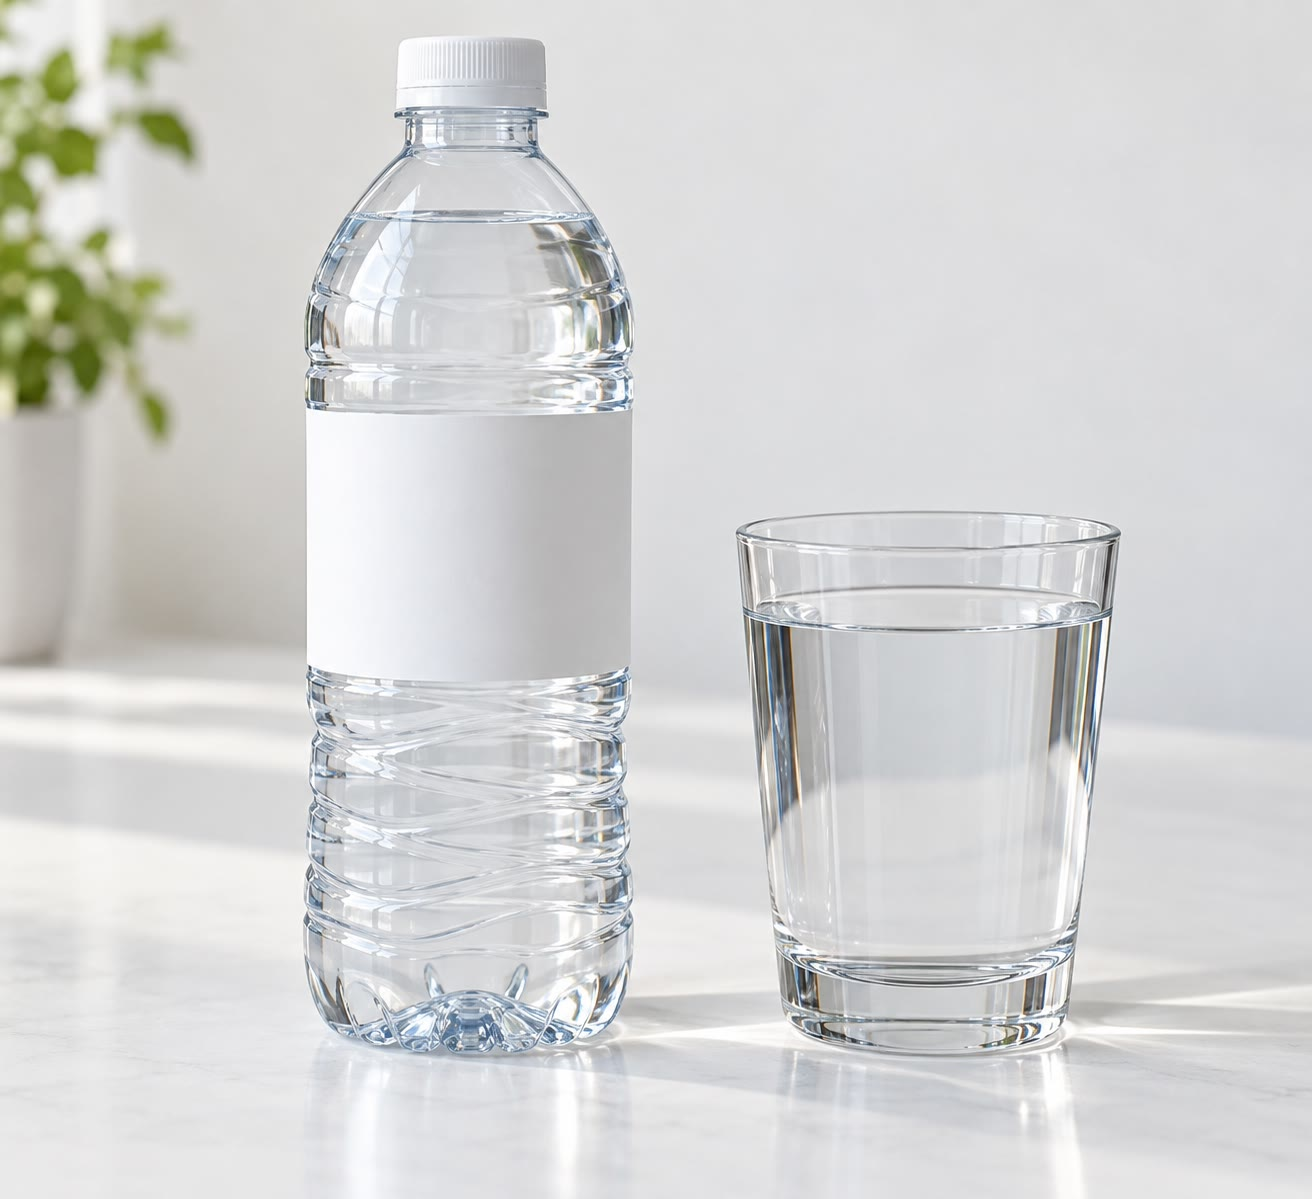
\includegraphics[width=0.5\linewidth]{images/book1/ai/g6-mineral-water.jpg}

{\small मिनरल वॉटर की एक बोतल: स्वच्छ और रंगहीन, फिर भी एक
\omterm{def:g6:pure-substances-and-mixtures:mixture}{मिश्रण}।}
\end{omfigure}

\begin{example}[मिनरल वॉटर का लेबल पढ़ना]\label{ex:g6:pure-substances-and-mixtures:label}
एक लेबल पर लिखा है: कैल्सियम \qty{78}{mg/L}, मैग्नीशियम \qty{24}{mg/L},
सोडियम \qty{5}{mg/L}, हाइड्रोजनकार्बोनेट \qty{357}{mg/L}, सल्फ़ेट
\qty{10}{mg/L}, क्लोराइड \qty{4}{mg/L}। (ये आँकड़े एक उदाहरण हैं।)
एक लीटर में $78 + 24 + 5 + 357 + 10 + 4 = 478$\,mg घुले हुए पदार्थ हैं,
लगभग आधा ग्राम: \qty{1000}{g} पानी के आगे बहुत कम,
पर उसे \omterm{def:g6:pure-substances-and-mixtures:mixture}{मिश्रण} बनाने के लिए काफ़ी।
\end{example}

\section{अभ्यास}

\begin{exercise}[$\star$]\label{exo:g6:pure-substances-and-mixtures:1}
\omterm{def:g6:pure-substances-and-mixtures:pure-substance}{शुद्ध पदार्थ} या \omterm{def:g6:pure-substances-and-mixtures:mixture}{मिश्रण}? आसुत जल, \omterm{def:g4:air-a-mixture-of-gases:air}{वायु}, समुद्र का पानी, शुद्ध लोहे का एक
टुकड़ा, दूध, चीनी का एक क्रिस्टल।
\end{exercise}

\begin{exercise}[$\star$]\label{exo:g6:pure-substances-and-mixtures:2}
समांगी या विषमांगी? नमकीन पानी, ग्रेनाइट, पानी पर तेल, नल का
पानी, मूसली।
\end{exercise}

\begin{exercise}[$\star$]\label{exo:g6:pure-substances-and-mixtures:3}
\omterm{def:g6:pure-substances-and-mixtures:species}{रासायनिक स्पीशीज़} क्या है? तीन उदाहरण दो।
\end{exercise}

\begin{exercise}[$\star$]\label{exo:g6:pure-substances-and-mixtures:4}
एक द्रव \qty{78}{\celsius} पर उबलता है, और उबलते समय उसका ताप
\qty{78}{\celsius} पर ही रहता है। स्थिरांकों की सारणी से अनुमान लगाओ कि
वह क्या है।
\end{exercise}

\begin{exercise}[$\star$]\label{exo:g6:pure-substances-and-mixtures:5}
रसायनज्ञ के लिए ``शुद्ध संतरे का रस'' \omterm{def:g6:pure-substances-and-mixtures:pure-substance}{शुद्ध पदार्थ} क्यों नहीं है?
\end{exercise}

\begin{exercise}[$\star\star$]\label{exo:g6:pure-substances-and-mixtures:6}
एक द्रव \qty{100.5}{\celsius} पर उबलना शुरू करता है और उबलते समय उसका ताप
बढ़ता है। क्या वह \omterm{def:g6:pure-substances-and-mixtures:pure-substance}{शुद्ध पदार्थ} है? वह क्या हो सकता है?
\end{exercise}

\begin{exercise}[$\star\star$]\label{exo:g6:pure-substances-and-mixtures:7}
चार बीकरों वाला चित्र देखो। किस बीकर में छन्ना \omterm{def:g6:pure-substances-and-mixtures:mixture}{मिश्रण} के हिस्सों को अलग कर
सकता है? किस बीकर में नहीं कर सकता?
\end{exercise}

\begin{exercise}[$\star\star$]\label{exo:g6:pure-substances-and-mixtures:8}
\qty{10}{cm^3} आयतन वाले धातु के एक घन का द्रव्यमान \qty{78.7}{g} है।
\qty{1}{cm^3} का द्रव्यमान कितना है? सारणी की कौन-सी धातु यह हो सकती है?
\end{exercise}

\begin{exercise}[$\star\star$]\label{exo:g6:pure-substances-and-mixtures:9}
उदाहरण वाले मिनरल वॉटर के लेबल से बताओ कि घुले हुए द्रव्यमान का कितना
प्रतिशत हाइड्रोजनकार्बोनेट है। निकटतम पूर्ण संख्या तक पूर्णांकित करो।
\end{exercise}

\begin{exercise}[$\star\star$]\label{exo:g6:pure-substances-and-mixtures:10}
समुद्र के पानी में प्रति किलोग्राम लगभग \qty{35}{g} लवण होते हैं। समुद्र के
पानी की \qty{2}{kg} की बाल्टी में लवणों का द्रव्यमान कितना है? समुद्र के पानी
के द्रव्यमान का कितना प्रतिशत लवण है?
\end{exercise}

\begin{exercise}[$\star\star\star$]\label{exo:g6:pure-substances-and-mixtures:11}
दो स्वच्छ, रंगहीन द्रव बिल्कुल एक जैसे दिखते हैं। प्रयोगशाला में किए जाने
वाले ऐसे दो मापन बताओ जो दिखाएँ कि वे एक ही \omterm{def:g6:pure-substances-and-mixtures:pure-substance}{शुद्ध पदार्थ} हैं
या नहीं।
\end{exercise}

\begin{exercise}[$\star\star\star$]\label{exo:g6:pure-substances-and-mixtures:12}
एक \omterm{def:g6:pure-substances-and-mixtures:mixture}{मिश्रण} \qty{90}{g} पानी और \qty{10}{g} एथेनॉल से बना है। उसके
द्रव्यमान का कितना प्रतिशत एथेनॉल है? क्या उसे स्थिरांकों की सारणी से पहचाना
जा सकता है? समझाओ।
\end{exercise}

\section{समस्या: तीन रंगहीन द्रव}

\begin{problem}[{सप्ताहांत समस्या --- स्वच्छ, रंगहीन द्रव से भरे तीन बिना
लेबल वाले फ़्लास्क, और वे मापन जो उन्हें अलग-अलग पहचानते हैं}]
\label{pb:g6:pure-substances-and-mixtures:1}
% ledger: bp:water, bp:ethanol, rho:water, rho:ethanol, rho:seawater, sea:salinity
एक प्रयोगशाला सहायक को तीन फ़्लास्क A, B और C मिलते हैं, जिनके लेबल
गिर चुके हैं। तीनों में एक स्वच्छ, रंगहीन द्रव है। प्रयोगशाला में ऐसे केवल
तीन द्रव इस्तेमाल होते हैं: आसुत जल, एथेनॉल, और एक क्षेत्र-भ्रमण से लाया गया
समुद्र का पानी। सहायक प्रयोगशाला में तीन तरह के
मापन करता है।

\medskip
\noindent\textbf{भाग I --- देखना।}
\begin{enumerate}
  \item तीनों द्रव बिल्कुल एक जैसे दिखते हैं। क्या सहायक देखकर बता सकता
        है कि कौन-से \omterm{def:g6:pure-substances-and-mixtures:pure-substance}{शुद्ध पदार्थ} हैं? समझाओ।
  \item अगर उनमें से एक \omterm{def:g6:pure-substances-and-mixtures:mixture}{मिश्रण} है, तो वह समांगी है या विषमांगी?
  \item किस तरह का मापन दिखा सकता है कि कोई द्रव \omterm{def:g6:pure-substances-and-mixtures:pure-substance}{शुद्ध
        पदार्थ} है?
\end{enumerate}

\medskip
\noindent\textbf{भाग II --- मापना।}
हर द्रव को उबलने तक गरम किया जाता है। द्रव A \qty{100}{\celsius} पर
उबलता है और उसका ताप वहीं टिका रहता है। द्रव B \qty{78}{\celsius} पर उबलता
है और वहीं टिका रहता है। द्रव C \qty{100.6}{\celsius} पर उबलना शुरू करता
है, और उसका ताप धीरे-धीरे बढ़ता ही जाता है। फिर हर द्रव के
\qty{50.0}{mL} तौले जाते हैं: A \qty{49.8}{g}, B
\qty{39.5}{g}, C \qty{51.2}{g}।
\begin{enumerate}[resume]
  \item कौन-से द्रव \omterm{def:g6:pure-substances-and-mixtures:pure-substance}{शुद्ध पदार्थ} हैं? कौन-सा \omterm{def:g6:pure-substances-and-mixtures:mixture}{मिश्रण} है?
  \item इस अध्याय की स्थिरांकों की सारणी की मदद से द्रव A और
        B के नाम बताओ।
  \item हर द्रव के \qty{1}{mL} (यानी \qty{1}{cm^3}) का द्रव्यमान
        निकालो।
  \item क्या ये द्रव्यमान प्रश्न 5 के तुम्हारे उत्तर से मेल खाते हैं?
  \item उबलते समय द्रव C का ताप बढ़ता क्यों जाता है?
\end{enumerate}

\medskip
\noindent\textbf{भाग III --- द्रव C में क्या है?}
द्रव C के \qty{100}{mL} को एक प्याली में सूखने के लिए छोड़ दिया जाता है। सारा
पानी उड़ जाने पर \qty{3.5}{g} सफ़ेद क्रिस्टल बचते हैं।
\begin{enumerate}[resume]
  \item यह अवशेष द्रव C के बारे में क्या दिखाता है?
  \item प्रश्न 6 में निकाले गए C के \qty{1}{mL} के द्रव्यमान से C के
        \qty{100}{mL} का द्रव्यमान निकालो, फिर उसके द्रव्यमान का कितना
        प्रतिशत नमक है (एक दशमलव स्थान तक)।
  \item समुद्र के पानी के हर किलोग्राम में लगभग \qty{35}{g} लवण होते हैं। यह
        कितना प्रतिशत है? प्रश्न 10 से तुलना करो।
  \item निष्कर्ष निकालो: द्रव C के हर लीटर में कितने ग्राम नमक है, और क्या
        द्रव C समुद्र का पानी है?
\end{enumerate}
\end{problem}
